\documentclass[12pt]{article}
\usepackage[utf8]{inputenc}
\usepackage[T2A]{fontenc}
\usepackage[russian]{babel}
\usepackage{amsmath,amssymb,amsfonts,tikz}
\usepackage{graphicx}
\usepackage{booktabs}
\usepackage{hyperref}
\usepackage[most]{tcolorbox}
\usepackage[style=verbose-ibid,backend=biber]{biblatex}
\addbibresource{references.bib}
\usepackage[margin=2.5cm]{geometry}
\usepackage{fancyhdr}
\pagestyle{fancy}
\fancyhf{}
\fancyhead[L]{Инструменты разделения редких ресурсов}
\fancyhead[R]{25 мин}
\fancyfoot[C]{\thepage}
\renewcommand{\headrulewidth}{0.4pt}

\title{\textbf{Инструменты разделения редких и неравномерно распределённых ресурсов}}
\author{}
\date{}

\begin{document}
\maketitle
\thispagestyle{fancy}

% ================= 1. ВВЕДЕНИЕ =================
\section{Введение: почему это не про «рынок или государство»}

Население хочет \textbf{тепло}, а не нефть. Спрос на нефть --- производный:
\begin{equation}\label{eq:derived}
D_{oil}(p) = \sum_{i=1}^{n} \alpha_i D_i(p_i),
\end{equation}
где $\alpha_i$ --- доля нефти в производстве конечного блага.

\textbf{Конкуренция} идёт на уровне:
\begin{itemize}
\item фирм (НПЗ, трейдеры, агроэкспорт),
\item государств (права на добычу, концессии, трансграничные воды).
\end{itemize}

Отсюда \textbf{ложная развилка} «рынок или государство». Инструментарий шире --- мы инвентаризируем его как инженеры.

% ================= 2. ТРИ ОСИ (с новым блоком) =================
\section{Три оси --- не путать}

\subsection{Ограниченность (flow / stock)}
Физический факт: \emph{потоковый} ресурс $\dot{Q} \le R$, \emph{запасовый} --- $Q_{total} \le S$.

\textbf{Индикатор:} горизонт исчерпания $R/Q$.

% Там же, где «Ограниченность»
\subsubsection{Водный стресс (Falkenmark)}
$$
WSI = \frac{\text{Total withdrawals}}{\text{Total renewable supply}}
$$
Пороги: $WSI<0.2$ — изобилие, $0.2<WSI<0.4$ — стресс, $WSI>0.4$ — редкость.
\textbf{Источник:} Falkenmark (1989), SIWI.

% После WSI
\subsection{Запас к добыче (Reserve-to-Production)}
$$
R/P = \frac{S}{\dot{Q}}
$$
Пороги: $R/P<20$ — сигнал (но не редкость!).
\textbf{Пример:} фосфаты — $R/P=150$ (1980) → пик ~2030.



\textbf{Важно:} если $R/Q \to \infty$ (поток), но $S(0) \le 0$ (нет избыточного спроса при нулевой цене) ---
\emph{инструменты распределения не нужны}.

\subsection{Редкость (scarcity)}
Экономическое понятие: $S = D(0) - Q$ --- избыточный спрос при нулевой цене.

% Раздел 2, подраздел «Редкость»
\subsubsection{Эластичность предложения}
$$
\eta = \frac{\Delta Q/Q}{\Delta p/p}
$$
$\eta \to 0$ — вертикальная кривая (редкость не снимается ценой).
\textbf{Пример:} нефть (в коротком периоде $\eta\approx 0.05$), органы ($\eta=0$).

\textbf{Параметры:}
\begin{itemize}
\item эластичность предложения,
\item наличие экономической ренты,
\item отношение запасы/добыча.
\end{itemize}

\textbf{Пример:} воздух в чистом месте --- $S(0) \le 0$ --- не редок; в мегаполисе --- редок.

\subsection{Неравномерность}
\textbf{Не то же, что редкость.} Это про ``где ресурс и у кого права''.
% Раздел 2, после «Неравномерность»
\subsubsection{Кривая Лоренца}
Пусть $F(x)$ — функция распределения доходов/прав, $F^{-1}(p)$ — квантильная функция.
Кривая Лоренца:
$$
L(p) = \frac{1}{\mu}\int_0^p F^{-1}(t)\,dt,\qquad p\in[0,1]
$$
Свойства: $L(0)=0$, $L(1)=1$, $L(p)\le p$.

% Сразу после Лоренца
\subsubsection{Индекс Джини (Gini)}
$$
G = 1 - 2\int_0^1 L(p)\,dp
   = \frac{\sum_{i=1}^n\sum_{j=1}^n |x_i-x_j|}{2n^2\mu}
$$
Интерпретация: доля пар, где большее значение у более богатого.
Пороги: $G<0.3$ — равномерное, $0.3<G<0.5$ — умеренное, $G>0.5$ — острое.

% После Джини
\subsubsection{Коэффициент вариации}
$$
CV = \frac{\sigma}{\mu}
$$
Пороги: $CV<0.3$ — слабая вариация, $0.3<CV<0.6$ — средняя, $CV>0.6$ — сильная.
\textbf{Плюс:} чувствителен к выбросам (в отличие от Джини).

% После CV (для институциональной концентрации)
\subsubsection{Индекс Херфиндаля–Хиршмана (HHI)}
Пусть $s_i$ — доля $i$-го держателя прав (в \%), $\sum s_i = 100$.
$$
HHI = \sum_{i=1}^N s_i^2
$$
Пороги (US DOJ): $HHI<1500$ — конкурентный, $1500<HHI<2500$ — умеренный, $HHI>2500$ — концентрированный.
\textbf{Пример:} вода Чили — $HHI=0.46$ (концентрация).



Три параметра:
\begin{enumerate}
\item \textbf{Геологическая концентрация} (доля запасов в топ-$N$ странах),
\item \textbf{Институциональная концентрация} (HHI по лицензиям) --- именно она у Перкинса,
\item \textbf{Неравномерность доступа по доходам} (Сен: голод --- не от нехватки еды, а от сбоя entitlement).
\end{enumerate}

\subsection{Ограниченность vs Редкость --- когда они расходятся}
\begin{itemize}
\item \textbf{Пастбище:} трава растёт с темпом $R$. Пока $R \ge$ изъятия --- система устойчива.
\item \textbf{То же пастбище:} если $D(0) > R$, даже при $R$ --- дефицит при нулевой цене.
\item \textbf{Воздух:} поток не ограничен, но $S(0) \le 0$ --- не редок.
\end{itemize}

\textbf{Вывод:} ограниченность --- необходимое, но не достаточное условие редкости.

% ================= 3. МАТРИЦА =================
\section{Матрица исключаемость / соперничество}

\begin{figure}[h]
\centering
\begin{tikzpicture}[scale=0.9]
\draw[->] (0,0) -- (6,0) node[right] {Исключаемость};
\draw[->] (0,0) -- (0,5) node[above] {Соперничество};
\draw[thick] (0,0) rectangle (3,3) node[midway] {Частные};
\draw[thick] (3,0) rectangle (6,3) node[midway] {Клубные};
\draw[thick] (0,3) rectangle (3,6) node[midway] {Общие (commons)};
\draw[thick] (3,3) rectangle (6,6) node[midway] {Открытый доступ};
\node at (1.5,1.5) {рынок};
\node at (4.5,1.5) {рынок / гос.};
\node at (1.5,4.5) {общинные правила};
\node at (4.5,4.5) {деградация};
\end{tikzpicture}
\caption{Четыре типа благ --- разные инструменты}
\end{figure}

\textbf{Ключевой вывод:} сам по себе ``общий'' ресурс --- не трагедия. Нужен \textbf{режим собственности} (Остром, 1990).

% ================= 4. ИНСТРУМЕНТАРИЙ =================
\section{Инструментарий --- три блока}

\subsection{Блок 1. Режимы собственности}
Частная, государственная, commons, открытый доступ.

\subsection{Блок 2. Механизмы распределения}
Аукцион (Vickrey), очередь, лотерея, переуступаемые квоты.

\subsection{Блок 3. Механизмы ограничения}
Налог Пигу, cap-and-trade, технологический лимит, правила самоуправления (8 условий Остром).

%================== 4.5 Дополнение =================
\begin{tabular}{@{}lccc@{}}
\toprule
\textbf{Благо / Инструмент} & \textbf{Рынок} & \textbf{Община / Квота} & \textbf{VCG / Гейл--Шепли} \\
\midrule
Нефть (частное)            & \checkmark & -- & -- \\
Спутник (клубное)          & \checkmark & -- & -- \\
Оборона (общественное)     & -- & \checkmark (налог) & \checkmark (опрос) \\
Пастбище (common)          & \checkmark (ITQ) & \checkmark (Остром) & -- \\
Вода (Чили)                & \checkmark (без потолка) & -- & -- \\
Вода (Австралия)           & -- & \checkmark (cap) & -- \\
Органы (UNOS)              & -- & -- & \checkmark (MELD/ГШ) \\
Антибиотики                & -- & \checkmark (stewardship) & -- \\
\bottomrule
\end{tabular}

% ================= 5. КЕЙС: ВОДА =================
\section{Кейс: вода --- Чили (1981) vs Австралия (Murray--Darling)}

\subsection{Чили}
Права отделены от земли, торгуемы, \textbf{нет потолка} \cite{bauer2004chile}. Результат: концентрация прав, падение стока Петорки до 50\% в засуху \cite{budds2008water}.

\subsection{Австралия}
$\bar{Q}$ --- экологически устойчивый объём, $q_i = e_i \cdot \bar{Q}/\sum e_i$ \cite{grafton2012water}. Результат: засуха 2000--2008 --- цена выросла втрое, \textbf{но объём $\le \bar{Q}$}, потери сельского хозяйства <1\%.

\subsection{Формальная разница}
\noindent % Убираем отступ абзаца в начале строки
\begin{minipage}[t]{0.45\textwidth} % [t] — выравнивание по верхнему краю 
\textbf{Чили:} $$q_i \ge 0,\quad \sum q_i \text{ не ограничен}$$ Цена $\to$ предельные издержки добычи. \end{minipage}\hfill% Заполняет пустое пространство между колонками 
\begin{minipage}[t]{0.45\textwidth} \textbf{Австралия:} $$\bar{Q} = \sum q_i,\quad q_i = e_i \cdot \frac{\bar{Q}}{\sum e_i}$$ Цена — рента за долю потолка. 
\end{minipage}

\textbf{Одна и та же конструкция (торгуемые права) $\Rightarrow$ противоположные результаты.}

% ================= 6. ВАЙЦМАН (ЦЕНА vs КОЛИЧЕСТВО) =================
\section{Правило Вайцмана (1974): цена vs количество}

\subsection{Модель}
Регулятор выбирает: \textbf{цена} (налог) или \textbf{количество} (квота).

При квадратичных потерях:
\begin{equation}\label{eq:weitzman}
\frac{L_{\text{price}}}{L_{\text{quota}}} = \left( \frac{e}{f} \right)^2,
\end{equation}
где $e$ --- наклон $MB$, $f$ --- наклон $MC$.

\subsection{Интерпретация}
\begin{itemize}
\item $e < f$ (MB пологая) $\Rightarrow$ \textbf{налог}.
\item $e > f$ (MB крутая) $\Rightarrow$ \textbf{квота}.
\item ``Толстые хвосты'' (Weitzman 2009) $\Rightarrow$ \textbf{квота}.
\end{itemize}

\subsection{Иллюстрация: углерод (Nordhaus 2018)}
\begin{figure}[h]
\centering
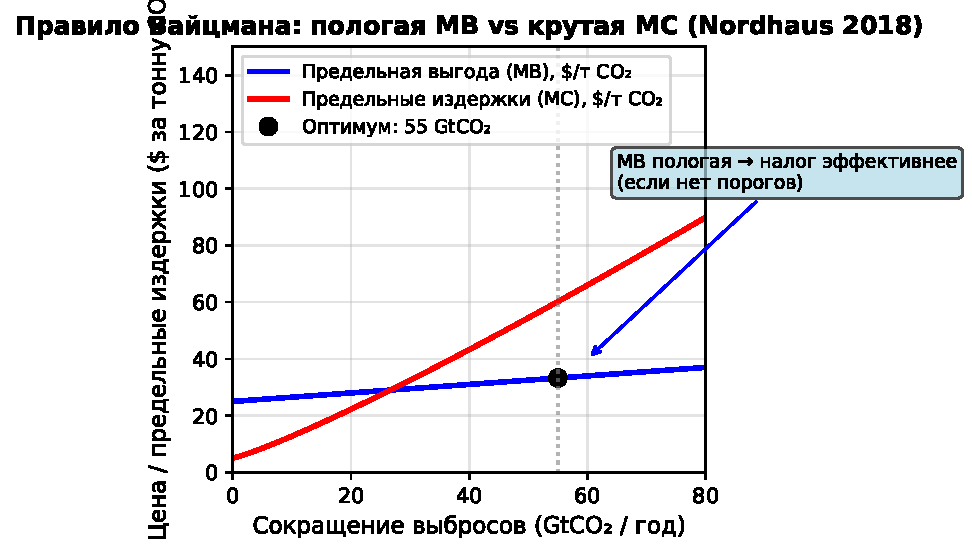
\includegraphics[width=0.9\linewidth]{nordhaus_mb_mc.pdf}
\caption{MB --- пологая, MC --- крутая. Оптимум $\approx 55$ $\text{GtCO}_2$/год, цена $\approx$ \$50--60/т \cite{nordhaus2018soccost}.}
\end{figure}

\section{Формальные механизмы: VCG и Гейл--Шепли}
\label{sec:vcg_gs}

\subsection{VCG — платежи за общественное благо}
\begin{equation}\label{eq:vcg}
x^*(\theta) = \arg\max_{x\in X} \sum_{i=1}^n v_i(x,\theta_i), \qquad
p_i(\theta) = \max_{x\in X} \sum_{j\neq i} v_j(x,\theta_j) - \sum_{j\neq i} v_j(x^*,\theta_j)
\end{equation}

\textbf{Пример:} три города, дорога A--B (стоимость 12). Выгода: A=8, B=6, C=0.
Платёж A = $0-6=-6$ (получает 6), платёж B = $0-8=-8$ (получает 8). Сумма платежей = 12.

\subsection{Гейл--Шепли — стабильное паросочетание}
\begin{itemize}
\item \textbf{Вход:} предпочтения $P(m_i), P(w_j)$.
\item \textbf{Алгоритм:} мужчины предлагают, женщины временно держат.
\item \textbf{Результат:} стабильно, мужско-оптимально, без денег.
\end{itemize}

\textbf{Пример 2$\times$2:} m1:w1>w2, m2:w2>w1; w1:m2>m1, w2:m1>m2. \\
Итог: $(m_1,w_1),(m_2,w_2)$ — нет блокирующих пар.

\subsection{Где применять}
\begin{itemize}
\item VCG — когда можно \textbf{оценить} индивидуальные выгоды (спутниковые данные, опросы), но нельзя организовать рынок.
\item Гейл--Шепли — когда \textbf{деньги запрещены} (органы, интерна, места в школах).
\end{itemize}

% ================= 7. UNOS — ТРЕТИЙ ПОЛЮС =================
\section{UNOS --- третий полюс: приоритизация без денег}

\subsection{MELD 3.0 (2023)}
Компоненты: билирубин, МНО, креатинин + диализ, пол ($+1.33$), HCC-исключения.

\subsection{Непрерывное распределение (2021--2023)}
Убраны границы DSA, расстояние --- компонент балла, баланс \textbf{срочность vs выживаемость}.

\textbf{Инструмент --- не рынок, не государство, а механизм приоритизации (балл).}

\subsection{Заменяемость органов --- почему не рынок}
У печени \textbf{нет backstop-технологии} (искусственная печень не масштабируется). Поэтому UNOS --- приоритизация, не аукцион. Если бы заменитель появился --- структура изменилась бы (как с CFC при озоновой дыре).

% ================= 8. ДРУГИЕ КЛАССЫ ИГР =================
\section{Что мы упустили: другие классы игр}

\subsection{Монголия --- commons $\to$ открытый доступ}
1990-е: приватизация скота, конец общинных правил. Поголовье: $\sim 25 \to 47$ млн (1990--2010). 70--88\% пастбищ деградированы \cite{worldbank2022mongolia}. \textbf{Провал:} не ``трагедия общин'', а разрушение работавшего института без замены.

\subsection{Антибиотики --- flow, не stock}
Общий ресурс --- \textbf{эффективность класса препаратов}. Каждый врач получает 100\% пользы сейчас, издержки --- на общество. Инструмент: stewardship (координация), не цена.

\subsection{Парадокс Браесса}
Добавление дороги $\Rightarrow$ рост времени в пути. Инструмент: congestion pricing (цена на внешний эффект), не квота.

\subsection{Банковская паника}
Игра без ресурса --- структура ожиданий. Инструмент: страхование вкладов (FDIC) --- \textbf{третий полюс}.

% ================= 9. ЗАМЕНЯЕМОСТЬ — КОГДА РЕСУРС ПЕРЕСТАЁТ БЫТЬ РЕДКИМ =================
\section{Заменяемость (backstop) --- когда редкость исчезает}

\subsection{Backstop и цена}
Если у ресурса есть \textbf{близкий заменитель} (substitute), при росте цены спрос переключается --- редкость не наступает.

\textbf{Формально:} если $\varepsilon \to \infty$, то $S(0) \le 0$ даже при конечном запасе.

\textbf{Примеры:}
\begin{itemize}
\item Озоновые дыры --- заменитель CFC появился \emph{до} катастрофы.
\item Нефть $\to$ электричество/биотопливо --- если backstop дешевле, Хотеллинг не работает.
\item Фосфор $\to$ рециклинг сточных вод (в отдельных регионах).
\end{itemize}

\subsection{Органы --- случай \textbf{ж} (нет заменителя)}
У печени и сердца \textbf{нет backstop}. Поэтому:
\begin{itemize}
\item рынок невозможен (этически и институционально),
\item остаётся \textbf{приоритизация} (UNOS),
\item при появлении искусственной печени --- система перейдёт к аукциону/цене (как CFC).
\end{itemize}

\textbf{Связь с Вайцманом:} крутая $MB$ (нет заменителя) $\Rightarrow$ квота/приоритизация, а не цена.

% ================= 10. СИНТЕЗ =================
\section{Синтез: какой инструмент --- когда?}

\begin{tabular}{@{}lll@{}}
\toprule
\textbf{Режим} & \textbf{Инструмент} & \textbf{Условие} \\
\midrule
Частная & Рынок & Спецификация прав \\
Государственная & Cap + trade & Измеримый потолок \\
Commons & Правила сообщества & Границы + мониторинг \\
Открытый доступ & --- & Не является институтом \\
\bottomrule
\end{tabular}
\vspace{0.5cm}

\textbf{Общий принцип:} \\
\textit{Инструмент следует из того, какой параметр вы можете измерить и удержать, \\
а не из названия ресурса.}

\textbf{Примеры:}
\begin{itemize}
\item вода (Чили) --- рынок (нет потолка),
\item вода (Австралия) --- cap + trade (есть потолок),
\item углерод --- налог ($e < f$), рядом порог --- квота,
\item органы --- приоритизация (нет backstop).
\end{itemize}

% ================= 11. ВОПРОС ЗАЛУ =================
\section{Вопрос залу}

На каком ресурсе вы бы \textbf{запретили} цену?
\begin{itemize}
\item вода,
\item органы,
\item радиочастоты,
\item углерод,
\item земля.
\end{itemize}

\vspace{1cm}
\begin{tcolorbox}{Основные источники}
Bauer (2004), Budds (2008), Grafton et al. (2012), Weitzman (1974), Nordhaus (2018), UNOS/OPTN Policy 4.0 (2023).
\end{tcolorbox}

\printbibliography
\end{document}
